
\begin{frame}
	\frametitle{Hierarchical Multipole Method}
	\begin{columns}
		\column{.7\textwidth}
			Central idea: use the multipole expansion of a distant group of particles to describe its gravity, instead of summing up the forces from all individual particles.			
			(For close groups, I use direct force calculation.)\\[1em]
			
			Multipole expansion of the potential gives:
			\begin{align*}
				\Phi(\mathbf{r}) &= -G \left( \frac{M}{|\mathbf{y}|} + \frac{1}{2} \frac{\mathbf{y}^T\mathbf{Q}\mathbf{y} }{\mathbf{|y|^5}} \right)\\
				\mathbf{y} &= \mathbf{r} - \mathbf{s}\\
				Q_{ij} &= \sum_k m_k [3(\mathbf{s} - \mathbf{x_k})_i(\mathbf{s} - \mathbf{x_k})_j - \delta_{ij} (\mathbf{s} - \mathbf{x_k})^2]
			\end{align*}
			
		\column{.3\textwidth}
			\centering
			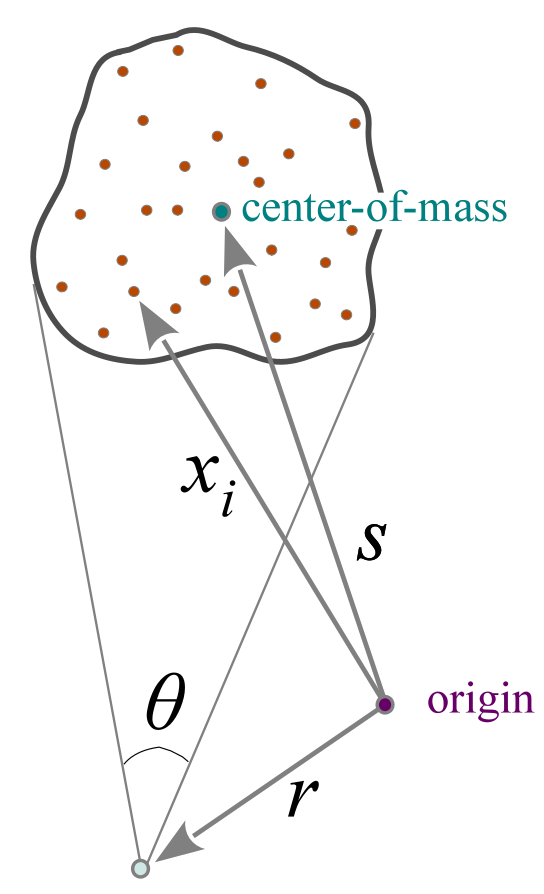
\includegraphics[width=\textwidth]{images/multipole.png} 
	\end{columns}

	The expansion is valid for $\theta \approx \frac{l}{y} \ll 1$
\end{frame}





\begin{frame}
	The particles are grouped hierarchically and the multipole moments are pre-computed for later use.
	
	I used the Barnes-Hut oct-tree: Assume particles are in a cube. The cube is then recursively subdivided into 8 sub-cubes of half the size in each spatial dimension, until each sub-cube contains only a single particle (or some other user-set limit).\\[1em]
	
	\textbf{Force calculation}: 
	
	For all leaf cells:
	
	\quad For all root cells:
	
	\quad\quad walk tree (this leaf cell, root cell)
	
	
	
\end{frame}




\begin{frame}
	\textbf{Walking the tree} (target cell, source cell):
	

	If source cell is leaf cell: Use direct force calculation, end walk for this source.
	
	If target (leaf) cell is inside this source cell:
	
	\quad for all children of the source cell:
	
	\quad \quad walk the tree (target, child of source)


	If target (leaf) cell is \textit{not} inside this source cell:
	
	\quad if $\theta < \theta_{max}$: Calculate multipole force, stop walk for this source
	
	\quad else: for all children of the source cell:
	
	\quad \quad walk the tree (target, child of source)
\end{frame}







\begin{frame}
	\begin{columns}
		\column{.33\textwidth}
			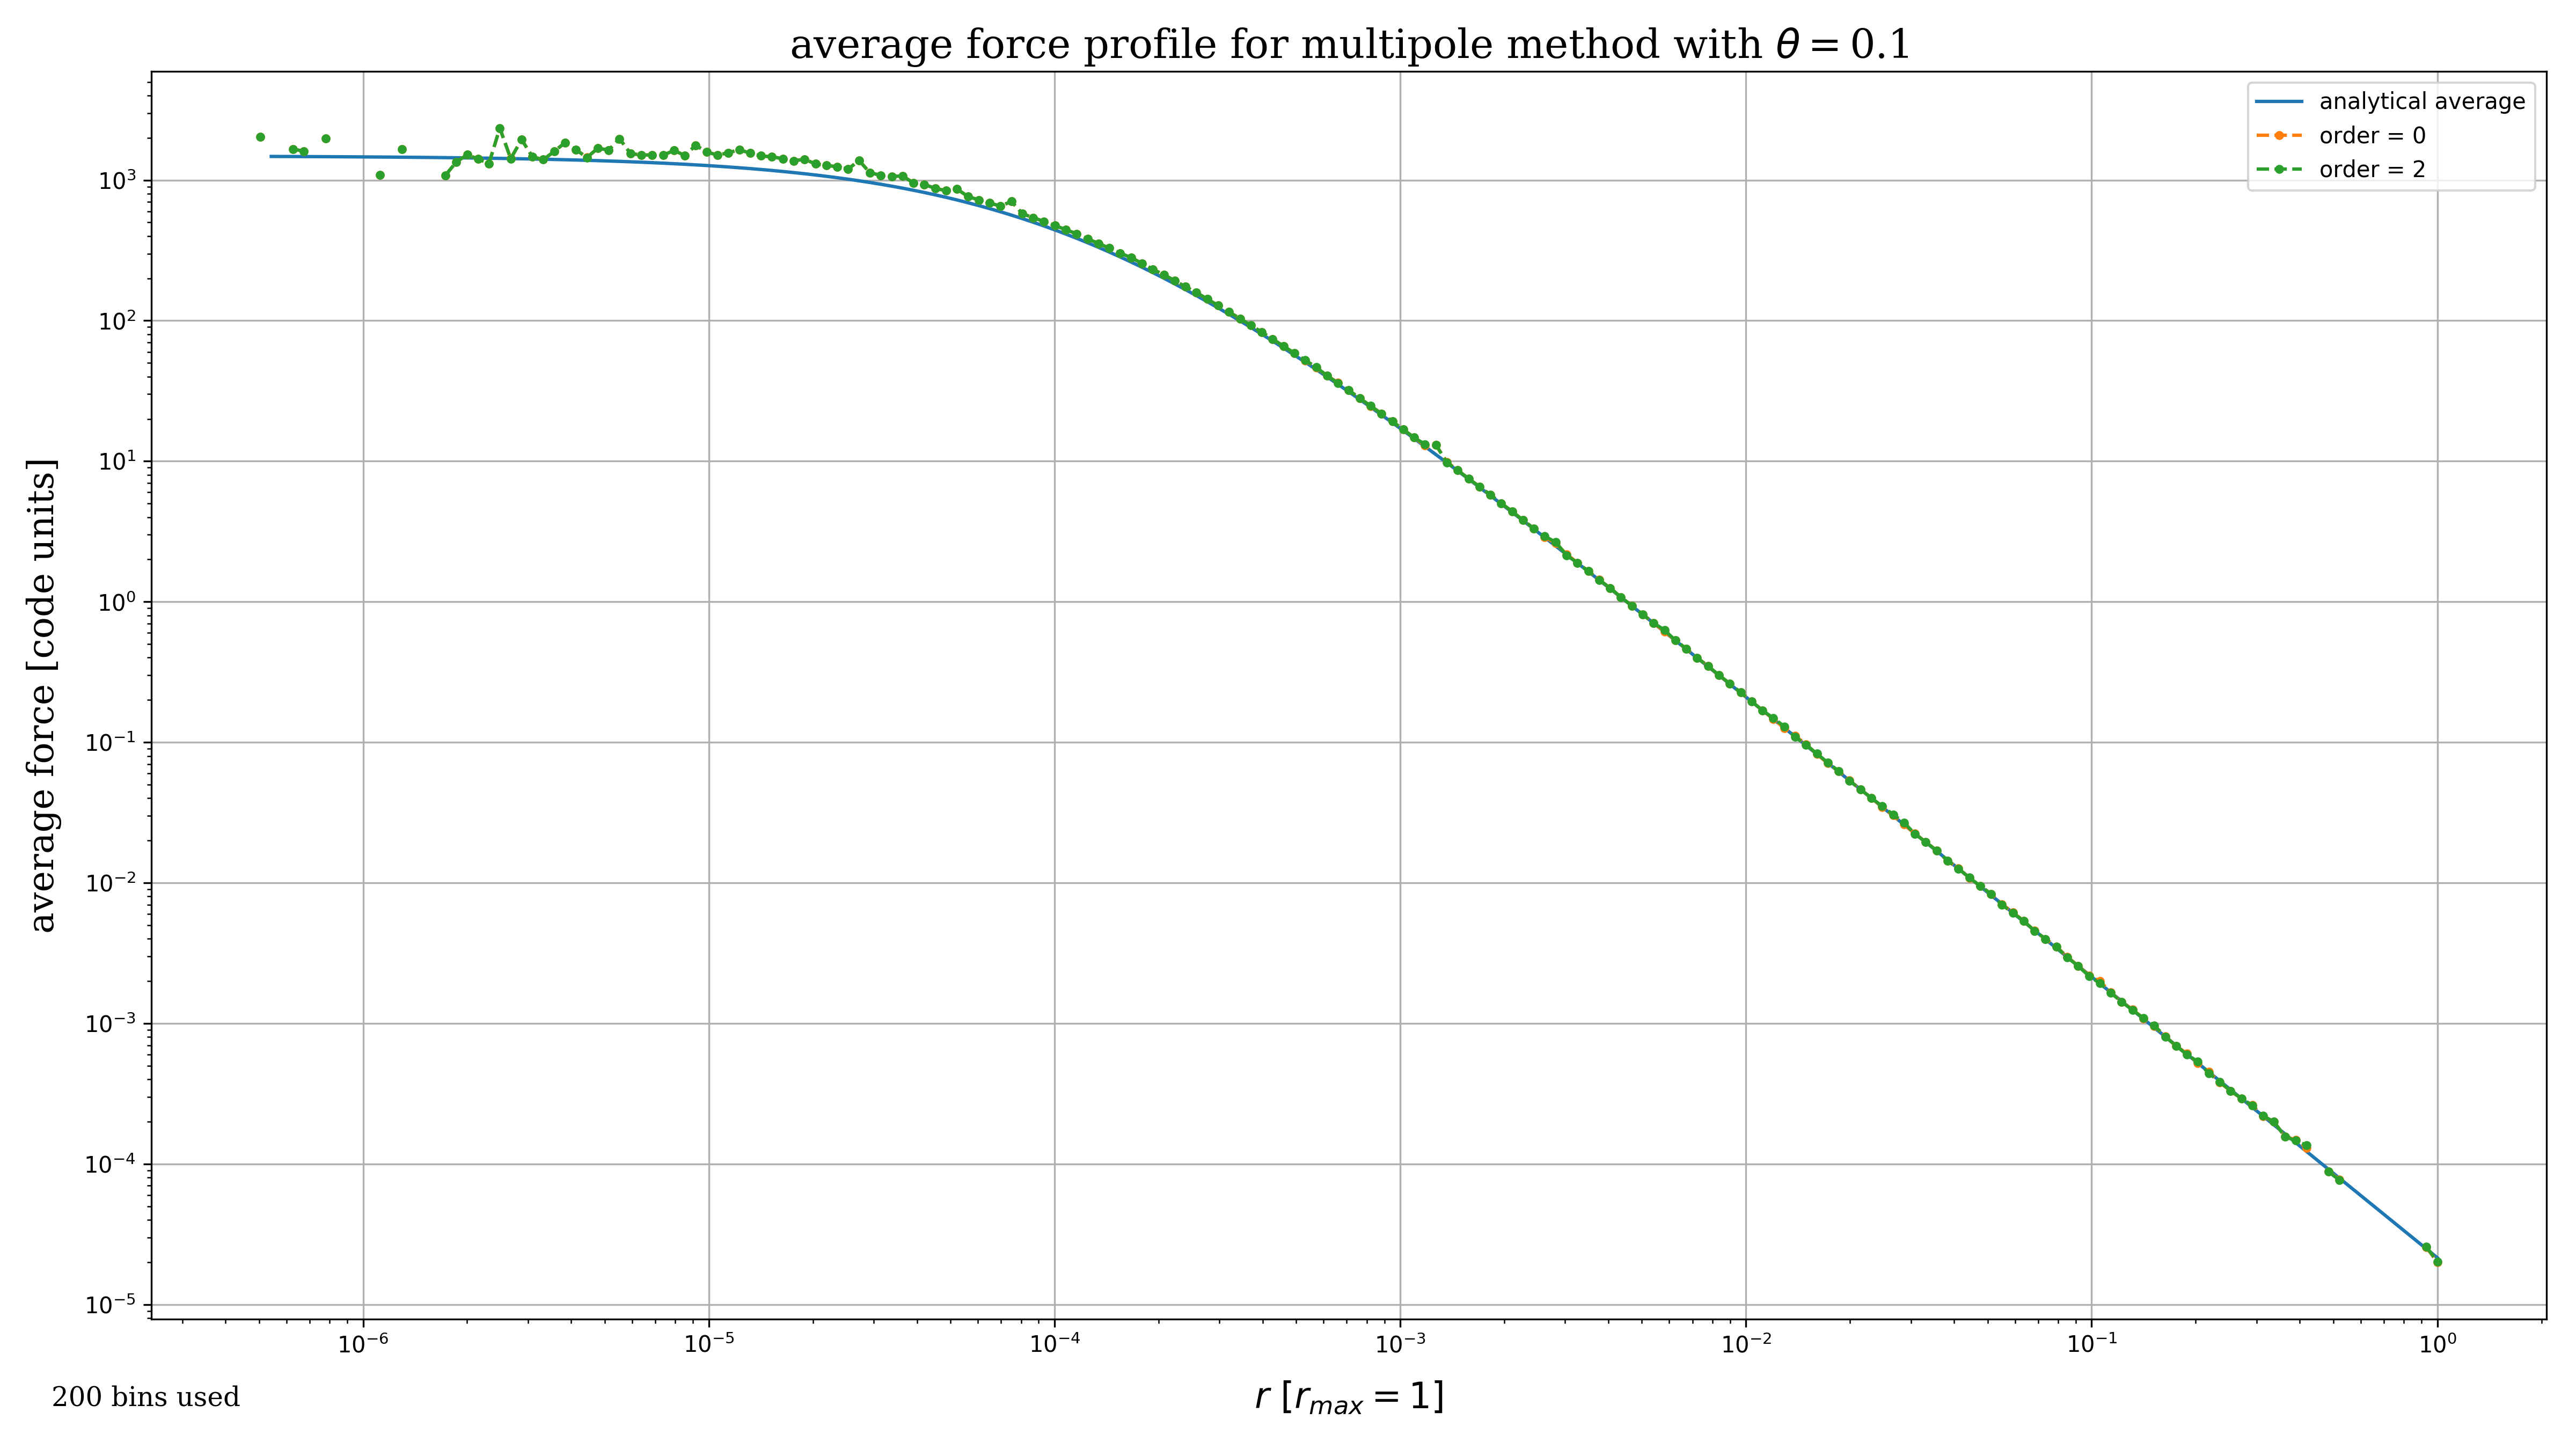
\includegraphics[width=\textwidth]{../results/multipole_forces/bucket01/0.1/multipole_forces_plot-0.1.png}\\[2em]
			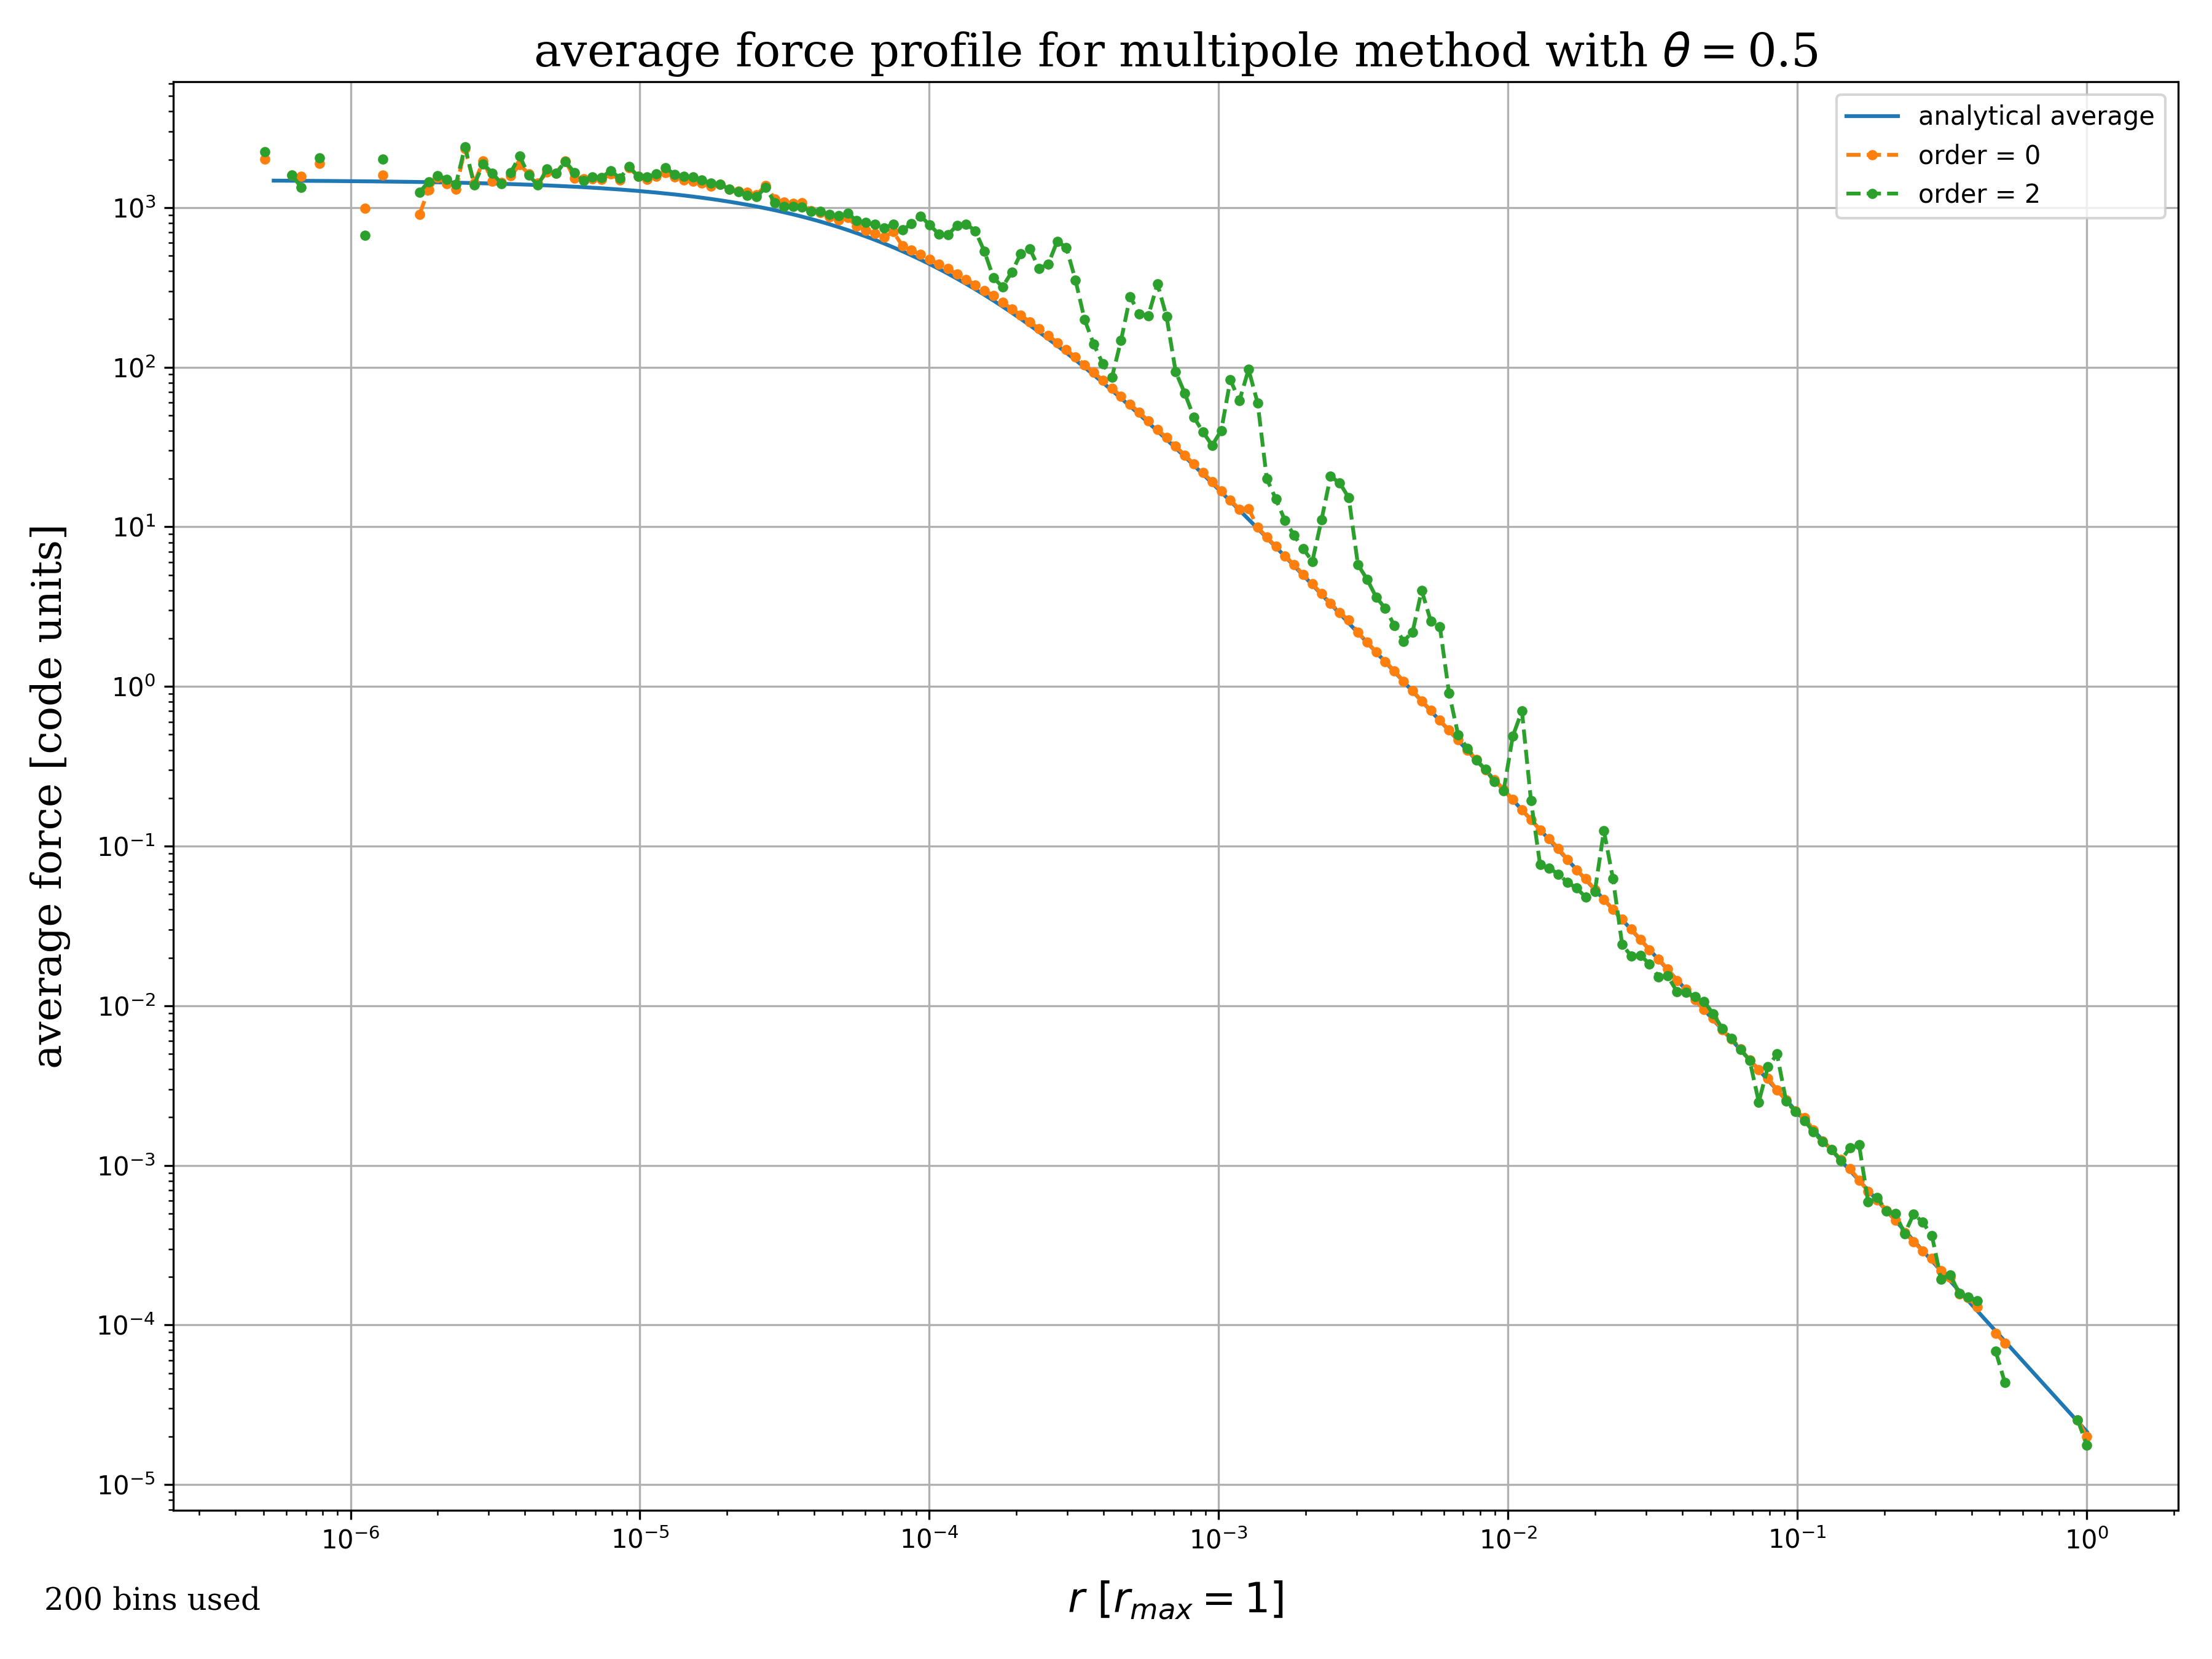
\includegraphics[width=\textwidth]{../results/multipole_forces/bucket01/0.5/multipole_forces_plot-0.5.png}
		\column{.33\textwidth}
			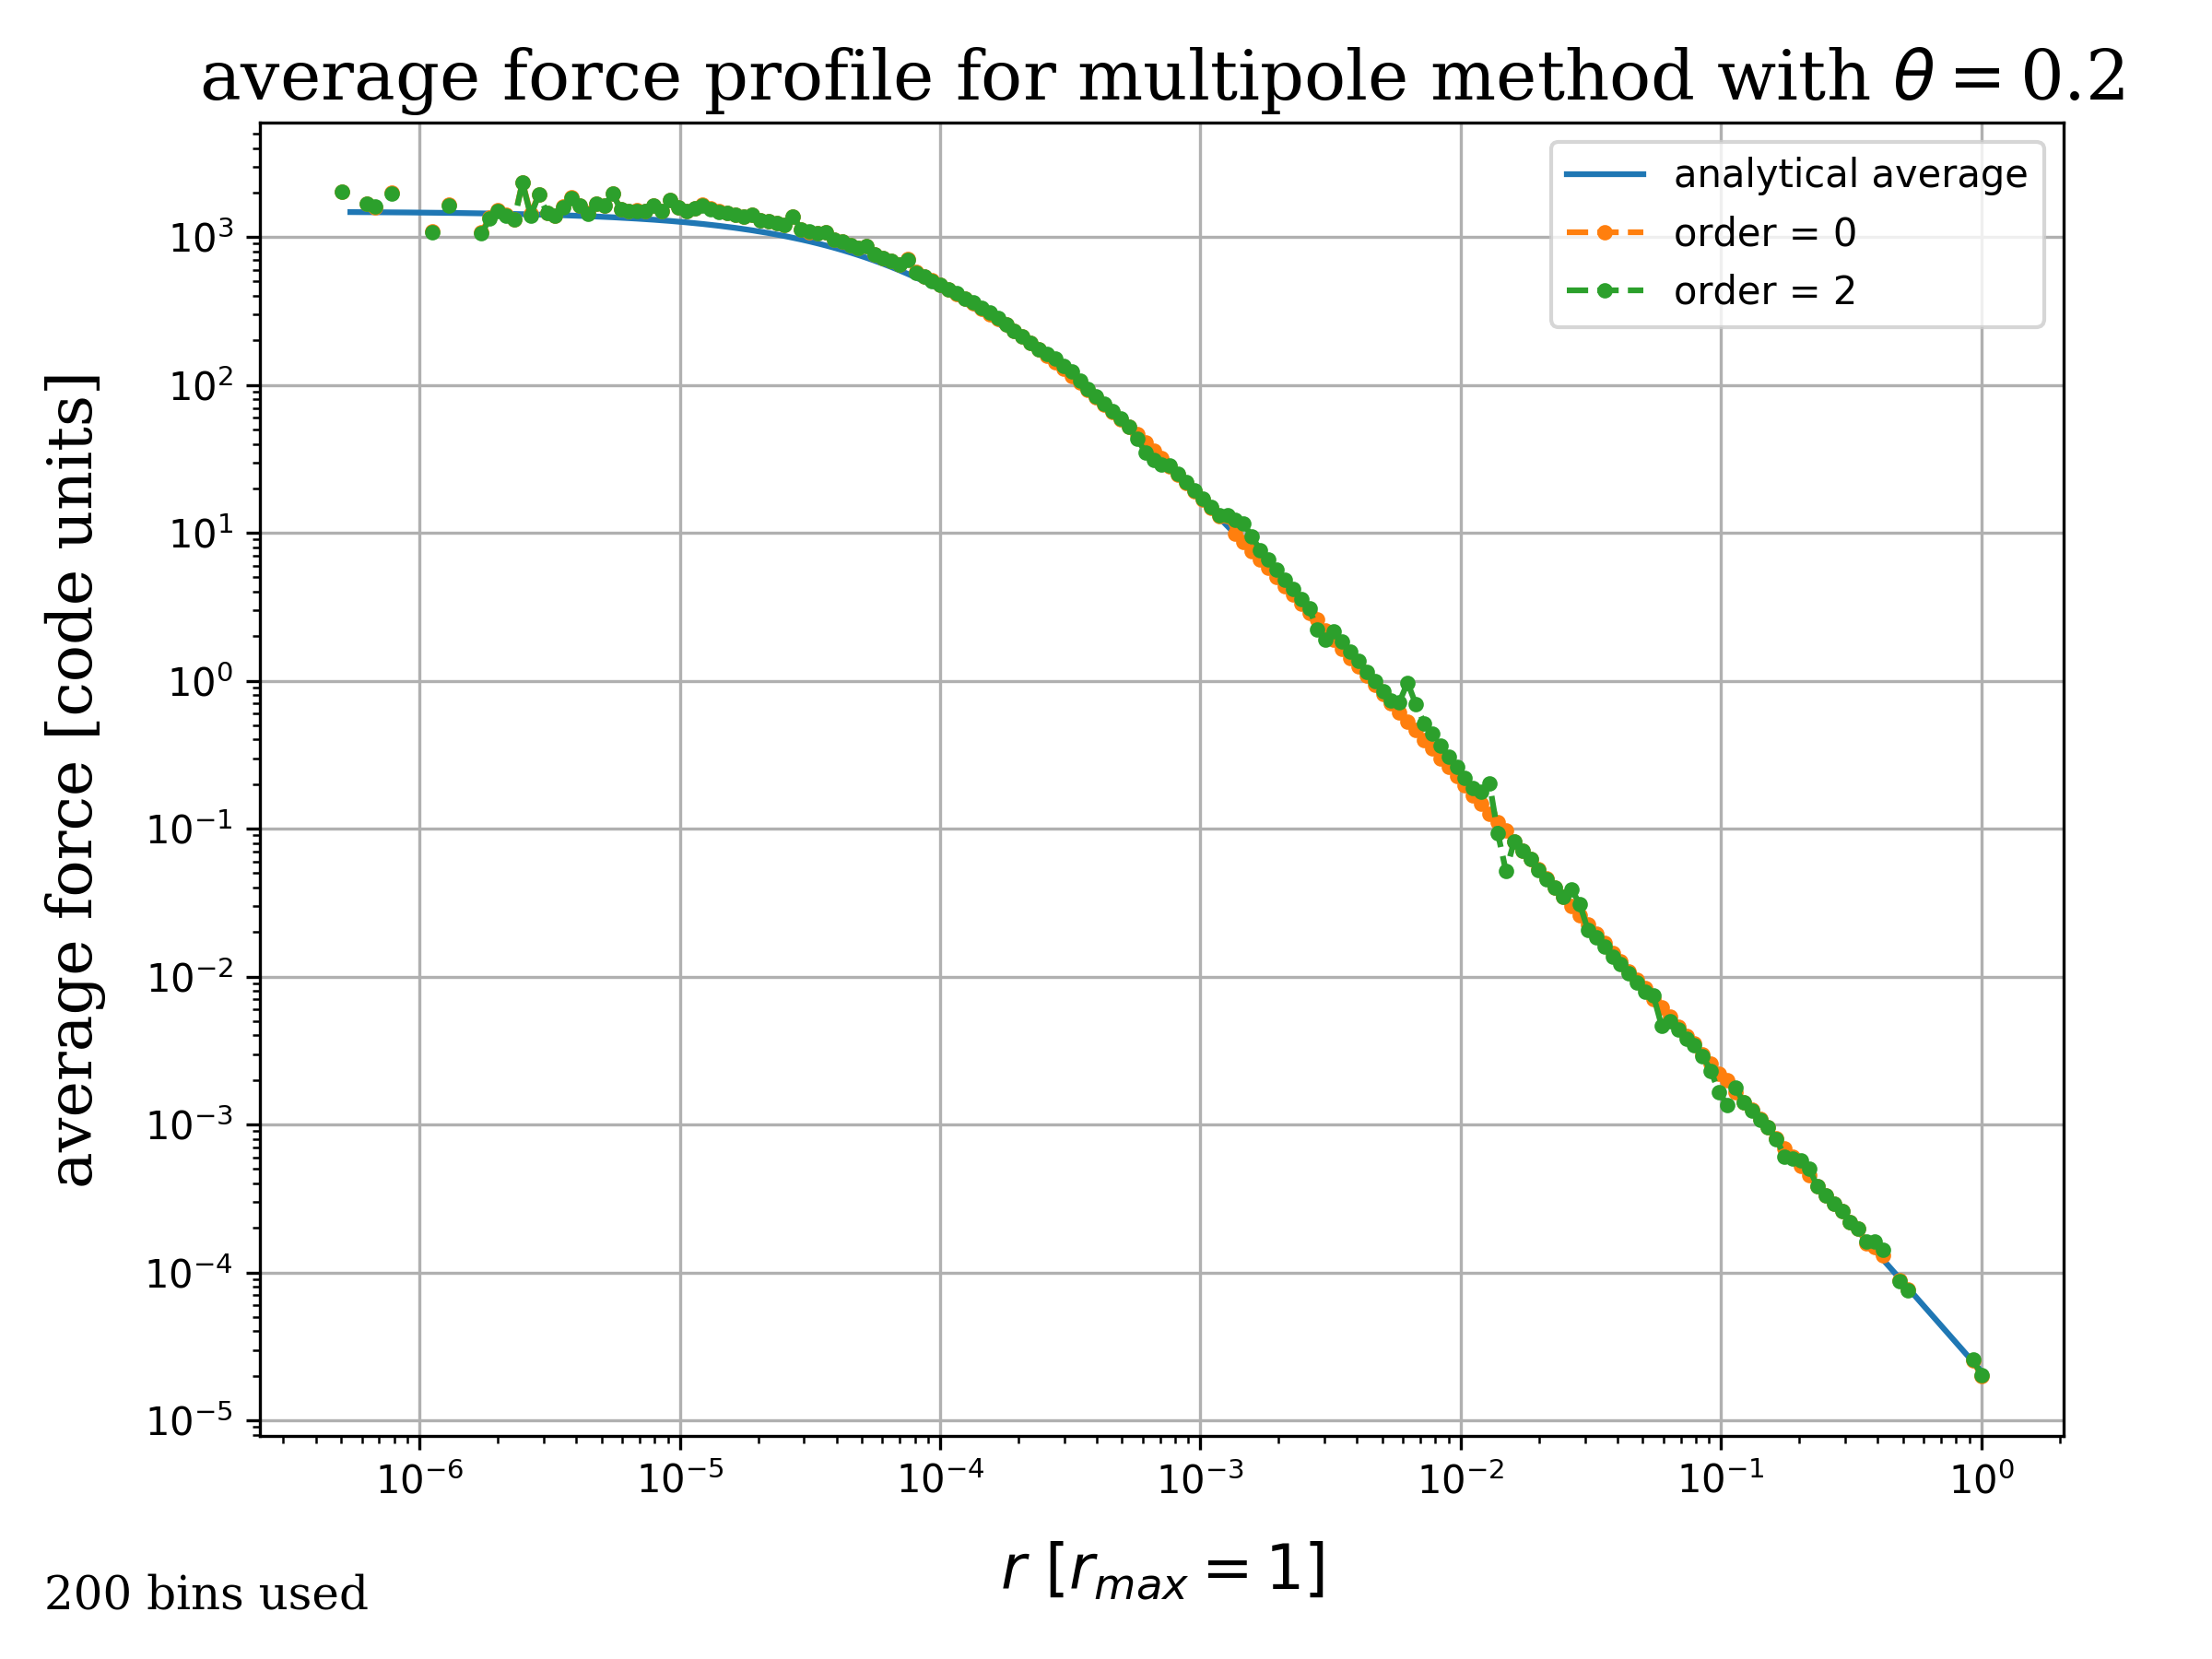
\includegraphics[width=\textwidth]{../results/multipole_forces/bucket01/0.2/multipole_forces_plot-0.2.png}\\[2em]
			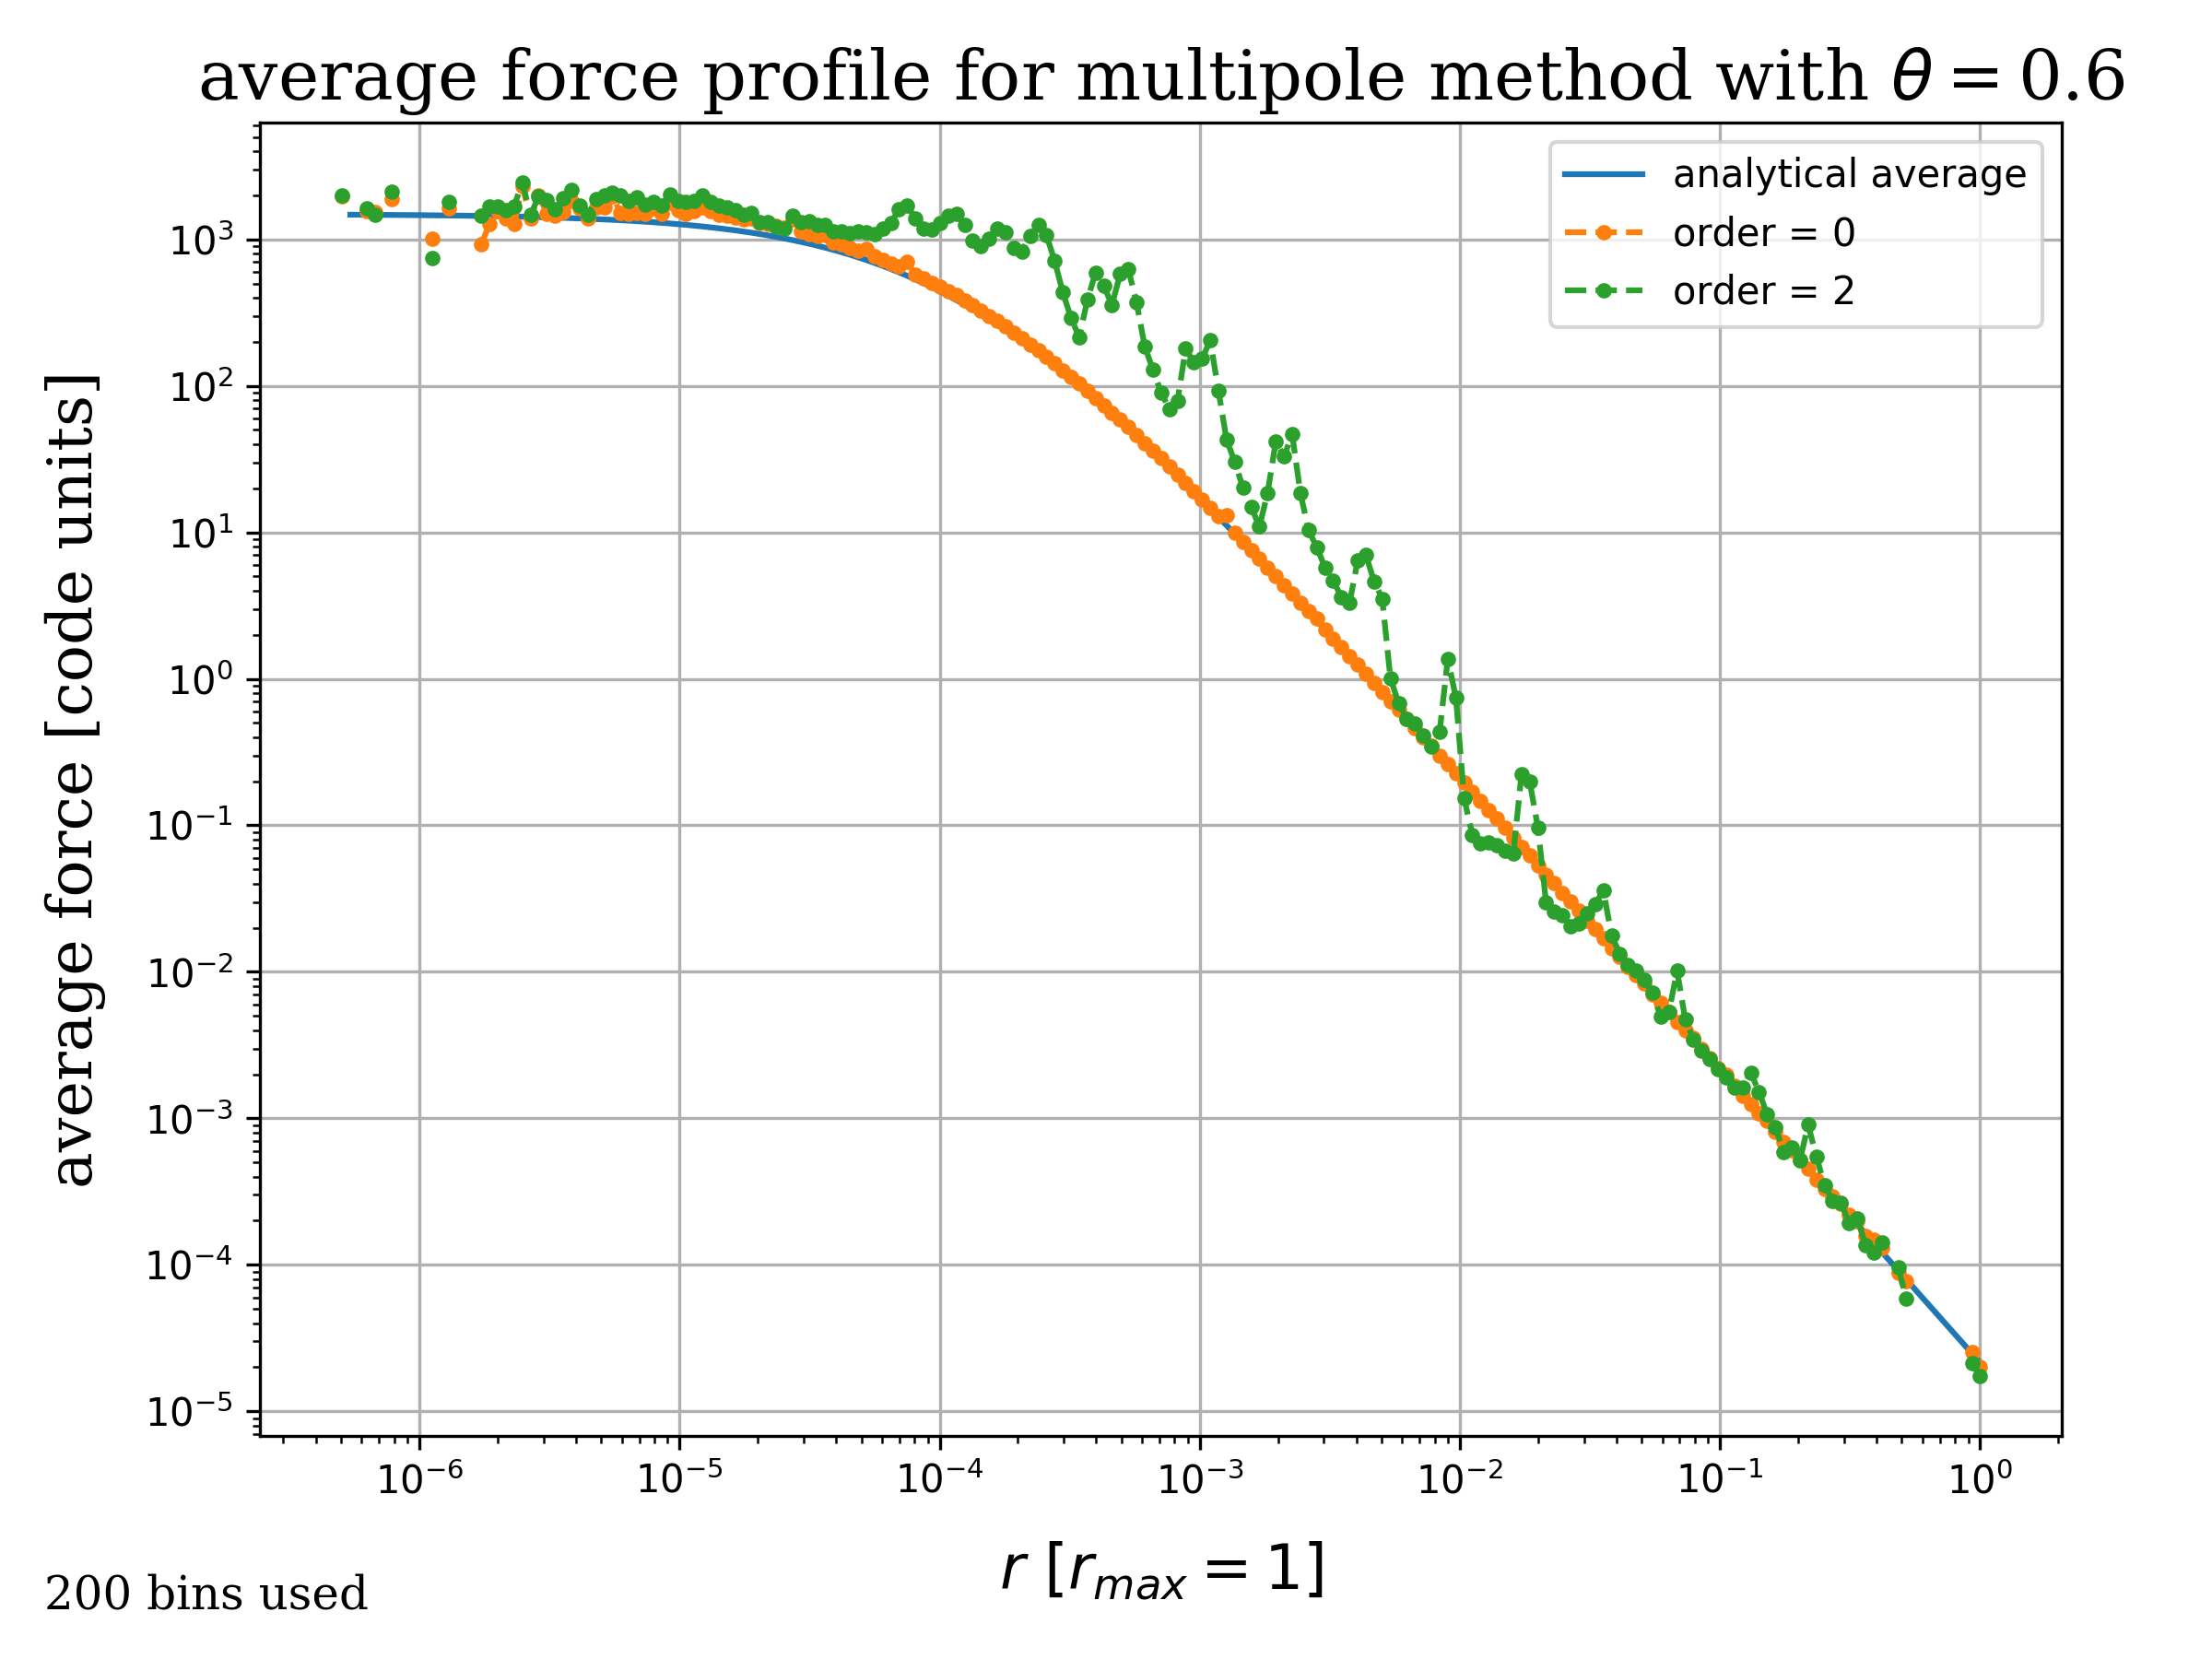
\includegraphics[width=\textwidth]{../results/multipole_forces/bucket01/0.6/multipole_forces_plot-0.6.png}
		\column{.33\textwidth}
			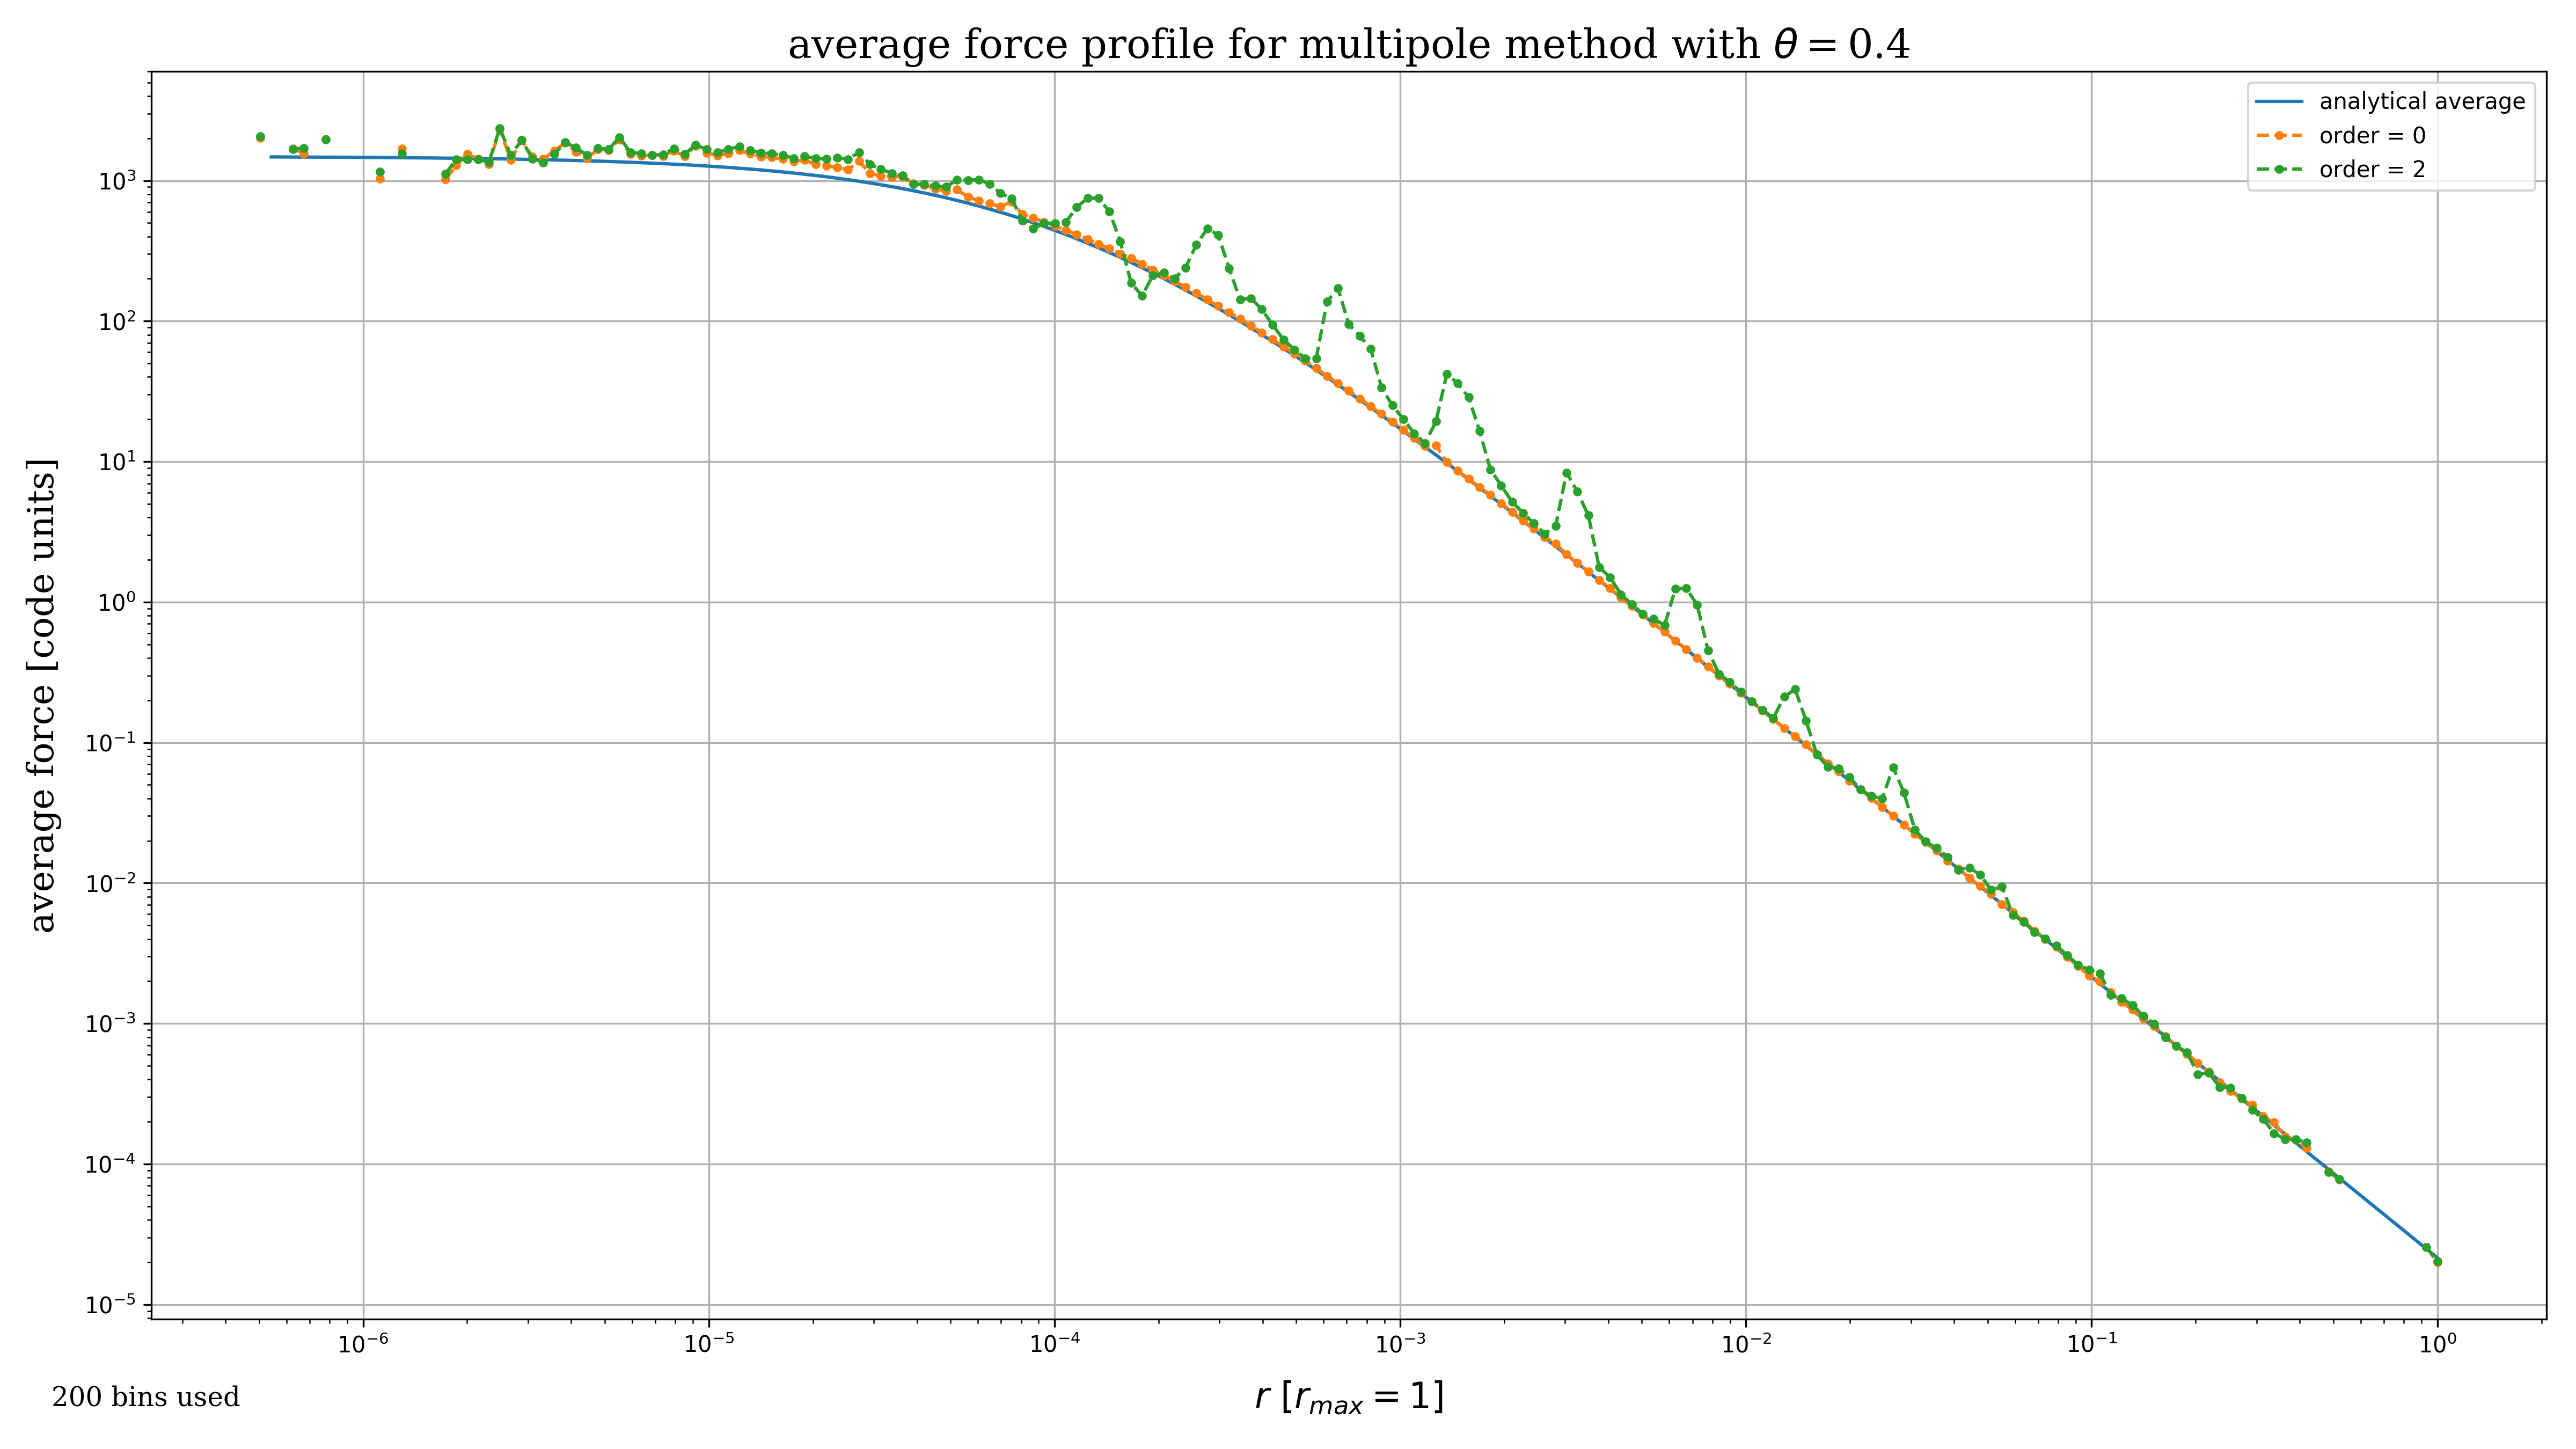
\includegraphics[width=\textwidth]{../results/multipole_forces/bucket01/0.4/multipole_forces_plot-0.4.png}\\[2em]
			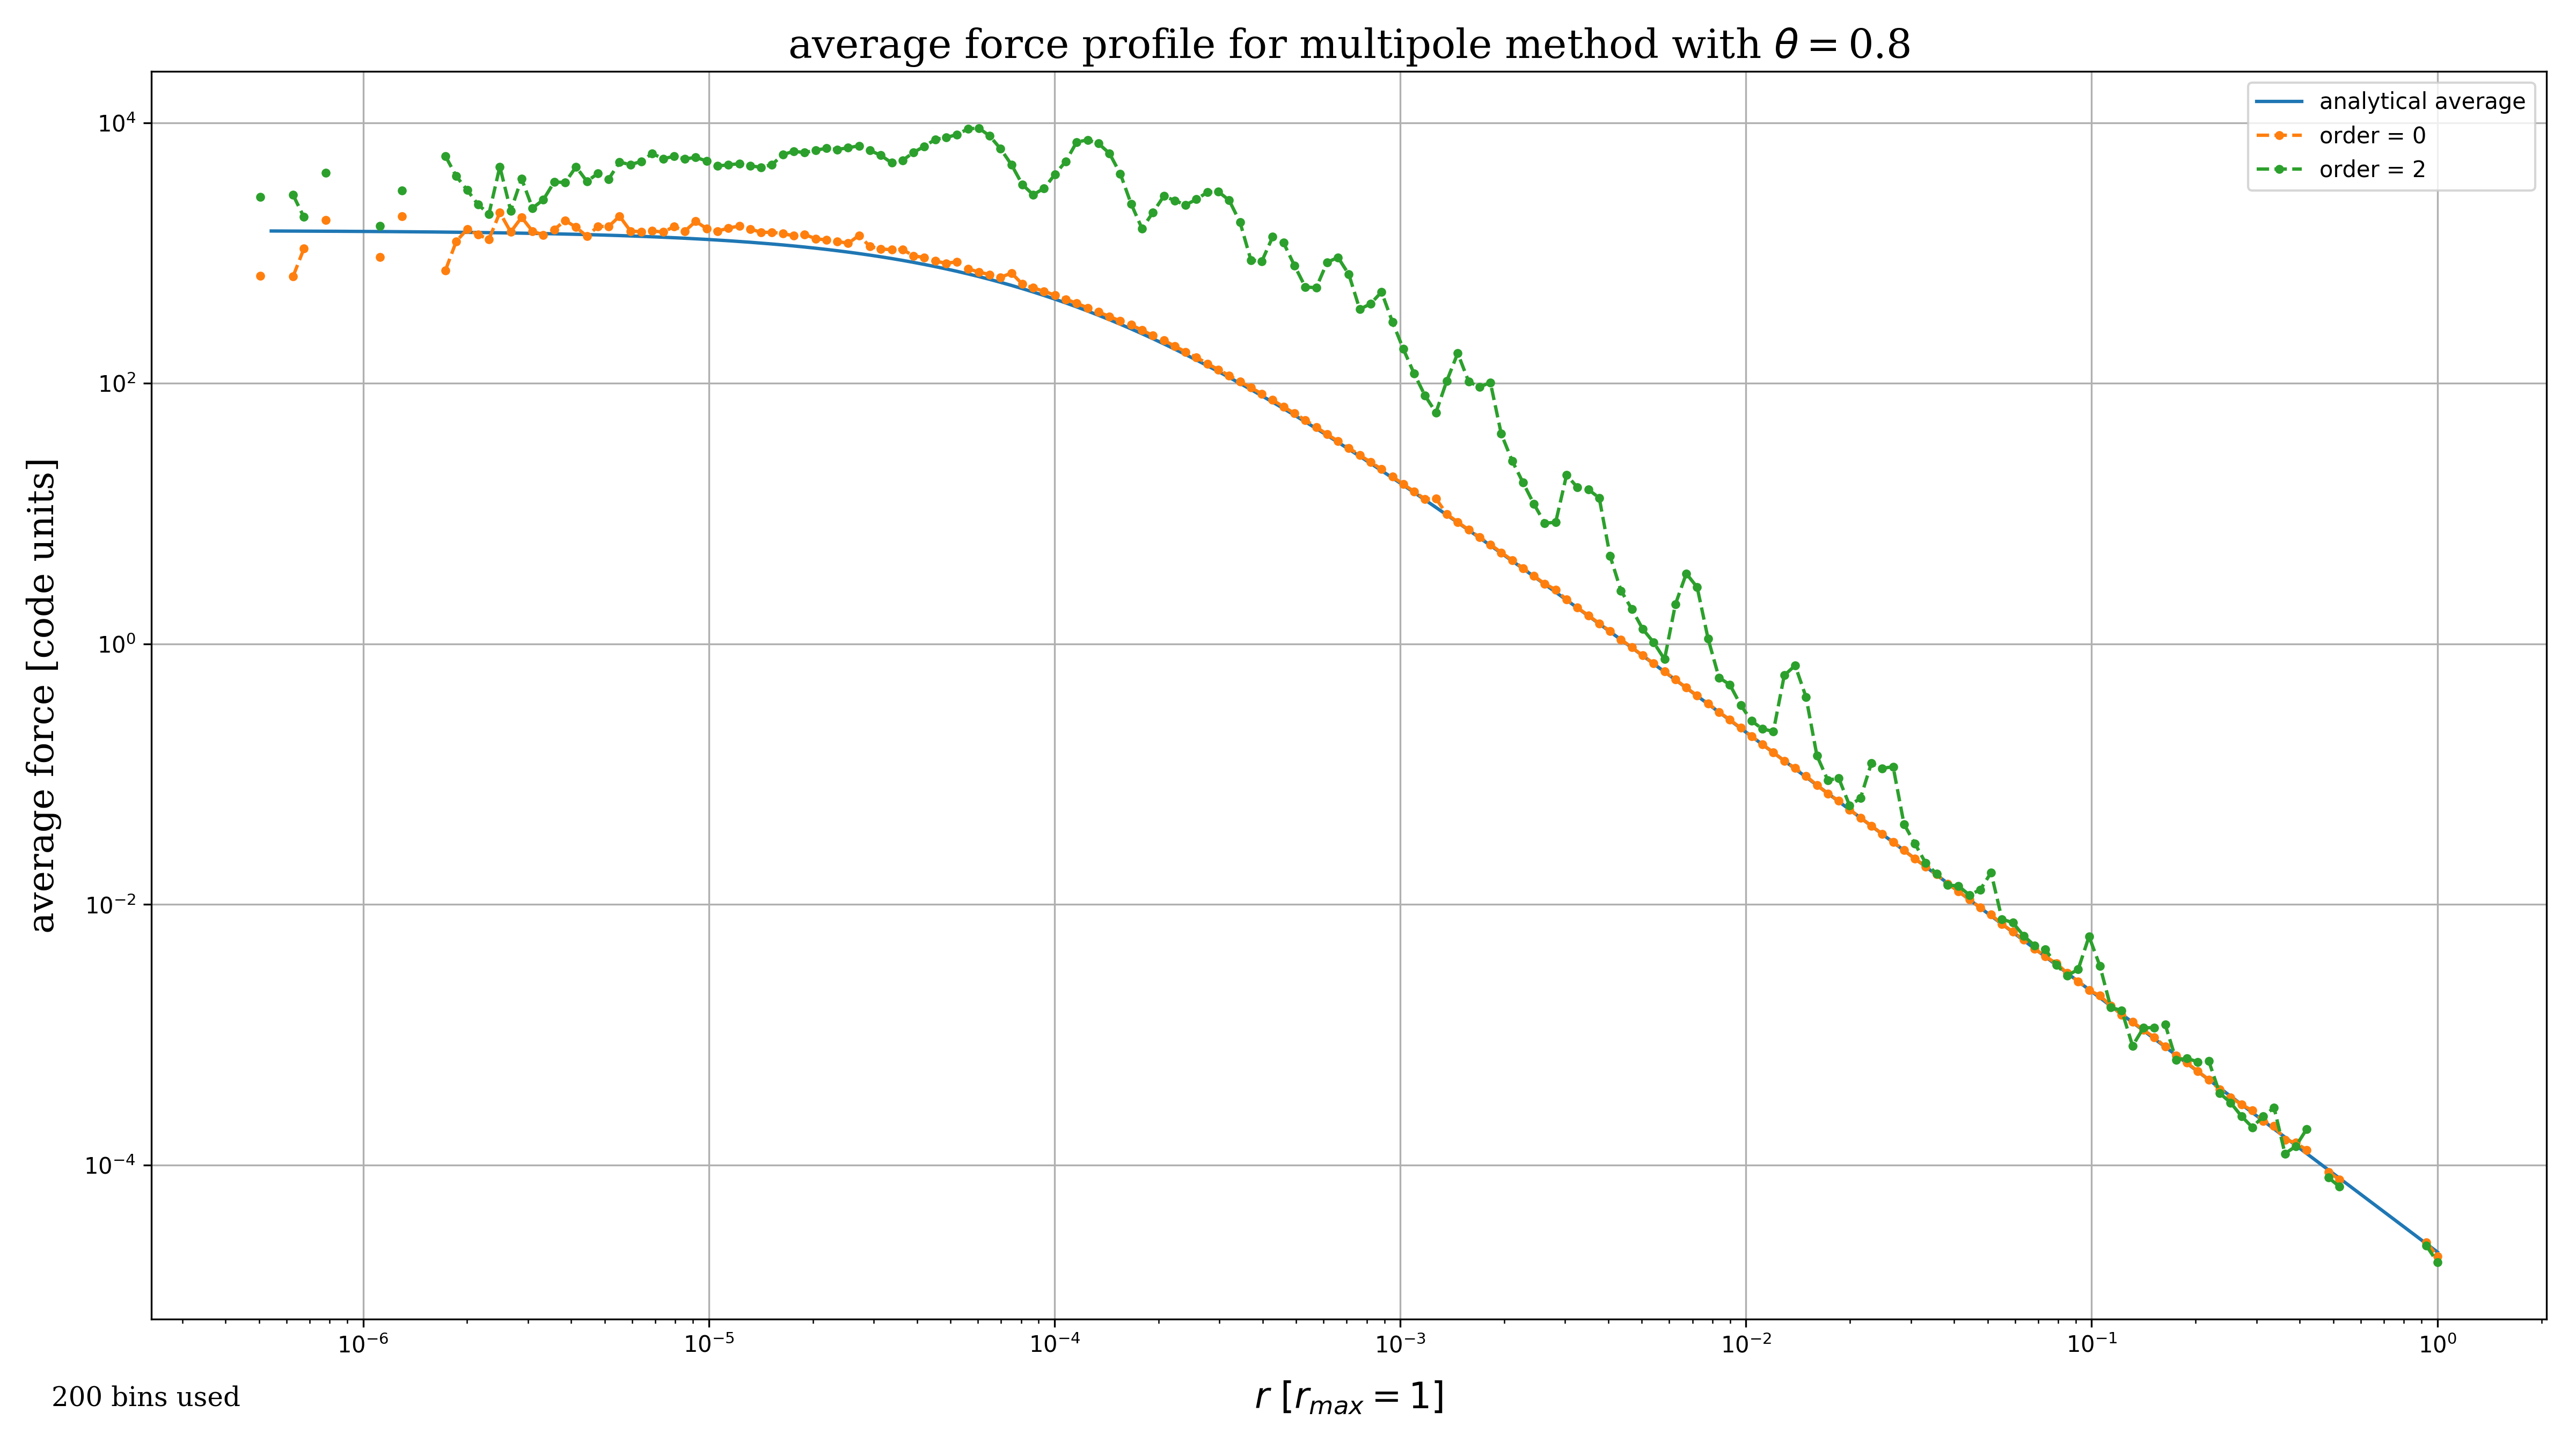
\includegraphics[width=\textwidth]{../results/multipole_forces/bucket01/0.8/multipole_forces_plot-0.8.png}
	\end{columns}
\end{frame}

